\chapter*{Dodatak: Prikaz aktivnosti grupe}
		\addcontentsline{toc}{chapter}{Dodatak: Prikaz aktivnosti grupe}
		
		\section*{Dnevnik sastajanja}
		
		\begin{packed_enum}

			\item  komunikacija - svakodnevna putem WhatsApp grupe
			\item[] \begin{packed_item}
				\item Datum: svakodnevno
				\item Prisustvovali: M. Dananić, P. Habjanec, D. Huić, V. Ivanić, L. Iveković, D. Ožvald, M. A. Stuhne
				\item Teme sastanka:
				\begin{packed_item}
					\item  napredak u područjima koda i dokumentacije
				\end{packed_item}
			\end{packed_item}

			\item  sastanak
			\item[] \begin{packed_item}
				\item Datum: 23.10.2023.
				\item Prisustvovali: M. Dananić, P. Habjanec, D. Huić, V. Ivanić, L. Iveković, D. Ožvald, M. A. Stuhne
				\item Teme sastanka:
				\begin{packed_item}
					\item  raspodjela posla
					\item  korištene tehnologije
					\item  initial commit
				\end{packed_item}
			\end{packed_item}
			
			\item  sastanak
			\item[] \begin{packed_item}
				\item Datum: 29.10.2023.
				\item Prisustvovali: M. Dananić, P. Habjanec, D. Huić, V. Ivanić, L. Iveković, D. Ožvald, M. A. Stuhne
				\item Teme sastanka:
				\begin{packed_item}
					\item  bitni zadatci do 2.11.2023.
					\item  dogovor oko dokumentacije
				\end{packed_item}
			\end{packed_item}
			
			%
			
		\end{packed_enum}
		
		\eject
		\section*{Tablica aktivnosti}
			\begin{longtblr}[
					label=none,
				]{
					vlines,hlines,
					width = \textwidth,
					colspec={X[7, l]X[1, c]X[1, c]X[1, c]X[1, c]X[1, c]X[1, c]X[1, c]}, 
					vline{1} = {1}{text=\clap{}},
					hline{1} = {1}{text=\clap{}},
					rowhead = 1,
				} 
			
				\SetCell[c=1]{c}{} & \SetCell[c=1]{c}{\rotatebox{90}{\textbf{Matija Alojz Stuhne}}} & \SetCell[c=1]{c}{\rotatebox{90}{\textbf{Marko Dananić }}} &	\SetCell[c=1]{c}{\rotatebox{90}{\textbf{Petra Habjanec }}} & \SetCell[c=1]{c}{\rotatebox{90}{\textbf{Dario Huić }}} &	\SetCell[c=1]{c}{\rotatebox{90}{\textbf{Valentina Ivanić }}} & \SetCell[c=1]{c}{\rotatebox{90}{\textbf{Luka Iveković }}} &	\SetCell[c=1]{c}{\rotatebox{90}{\textbf{Dominik Ožvald }}} \\  
				Backend			& + &  &  & + &  & + \\
				Frontend			& &  & + & + & + & & + \\
				Dokumentacija			& + & + & + & + &  & \\
				Prezentacija 			&  & + &  &  &  &  & \\  
				&  &  &  &  &  &  &  \\ \hline 
			\end{longtblr}
					
					
		\eject
		\section*{Dijagrami pregleda promjena}
		\begin{figure}[H]
			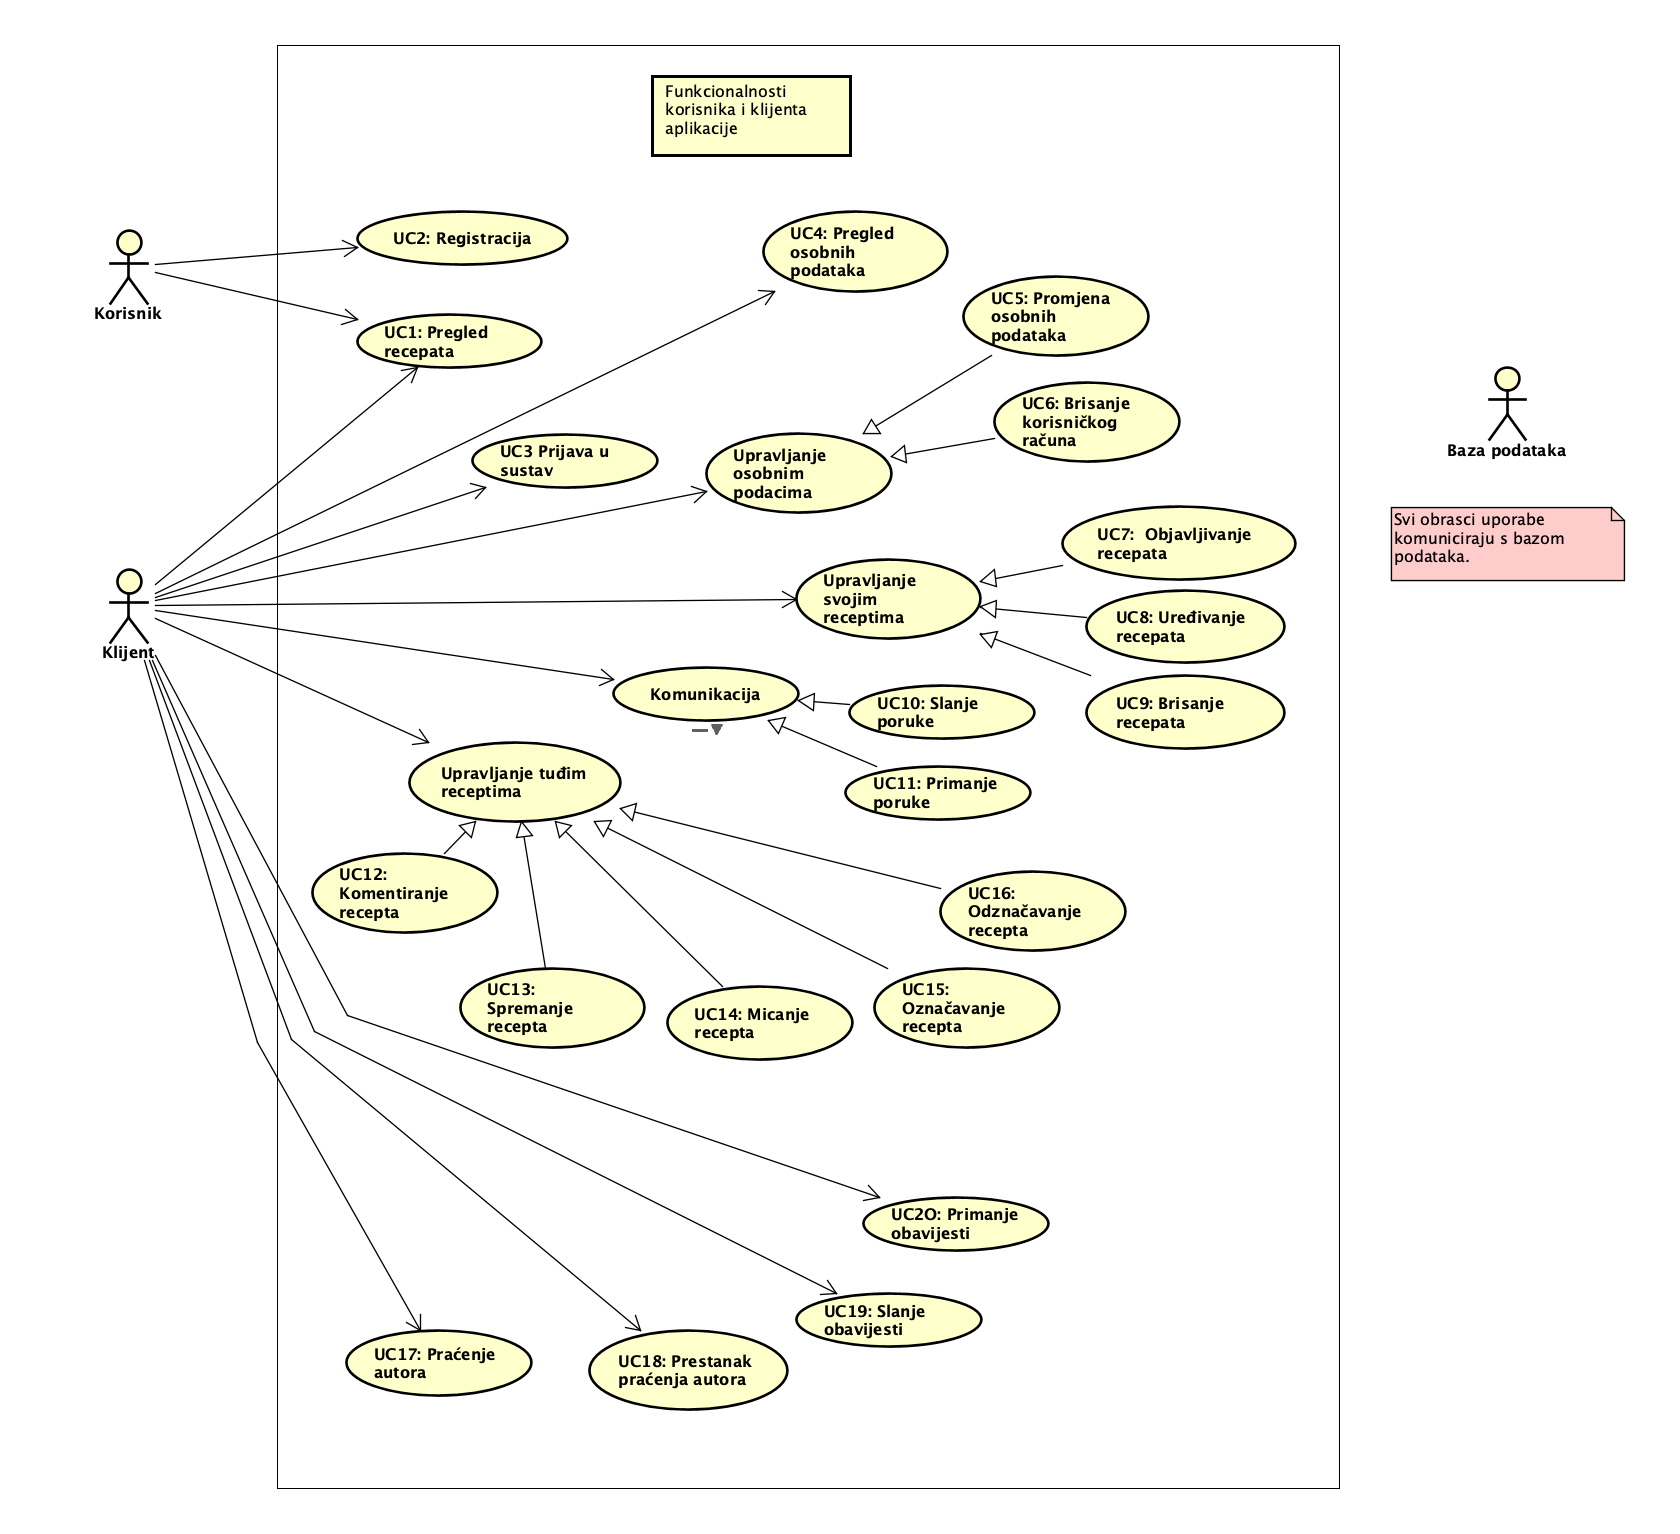
\includegraphics[scale=0.1]{dijagrami/Korisnik_klijent.png} 
			\centering
			\caption{}
			\label{fig:all}
		\end{figure}
		\begin{figure}[H]
			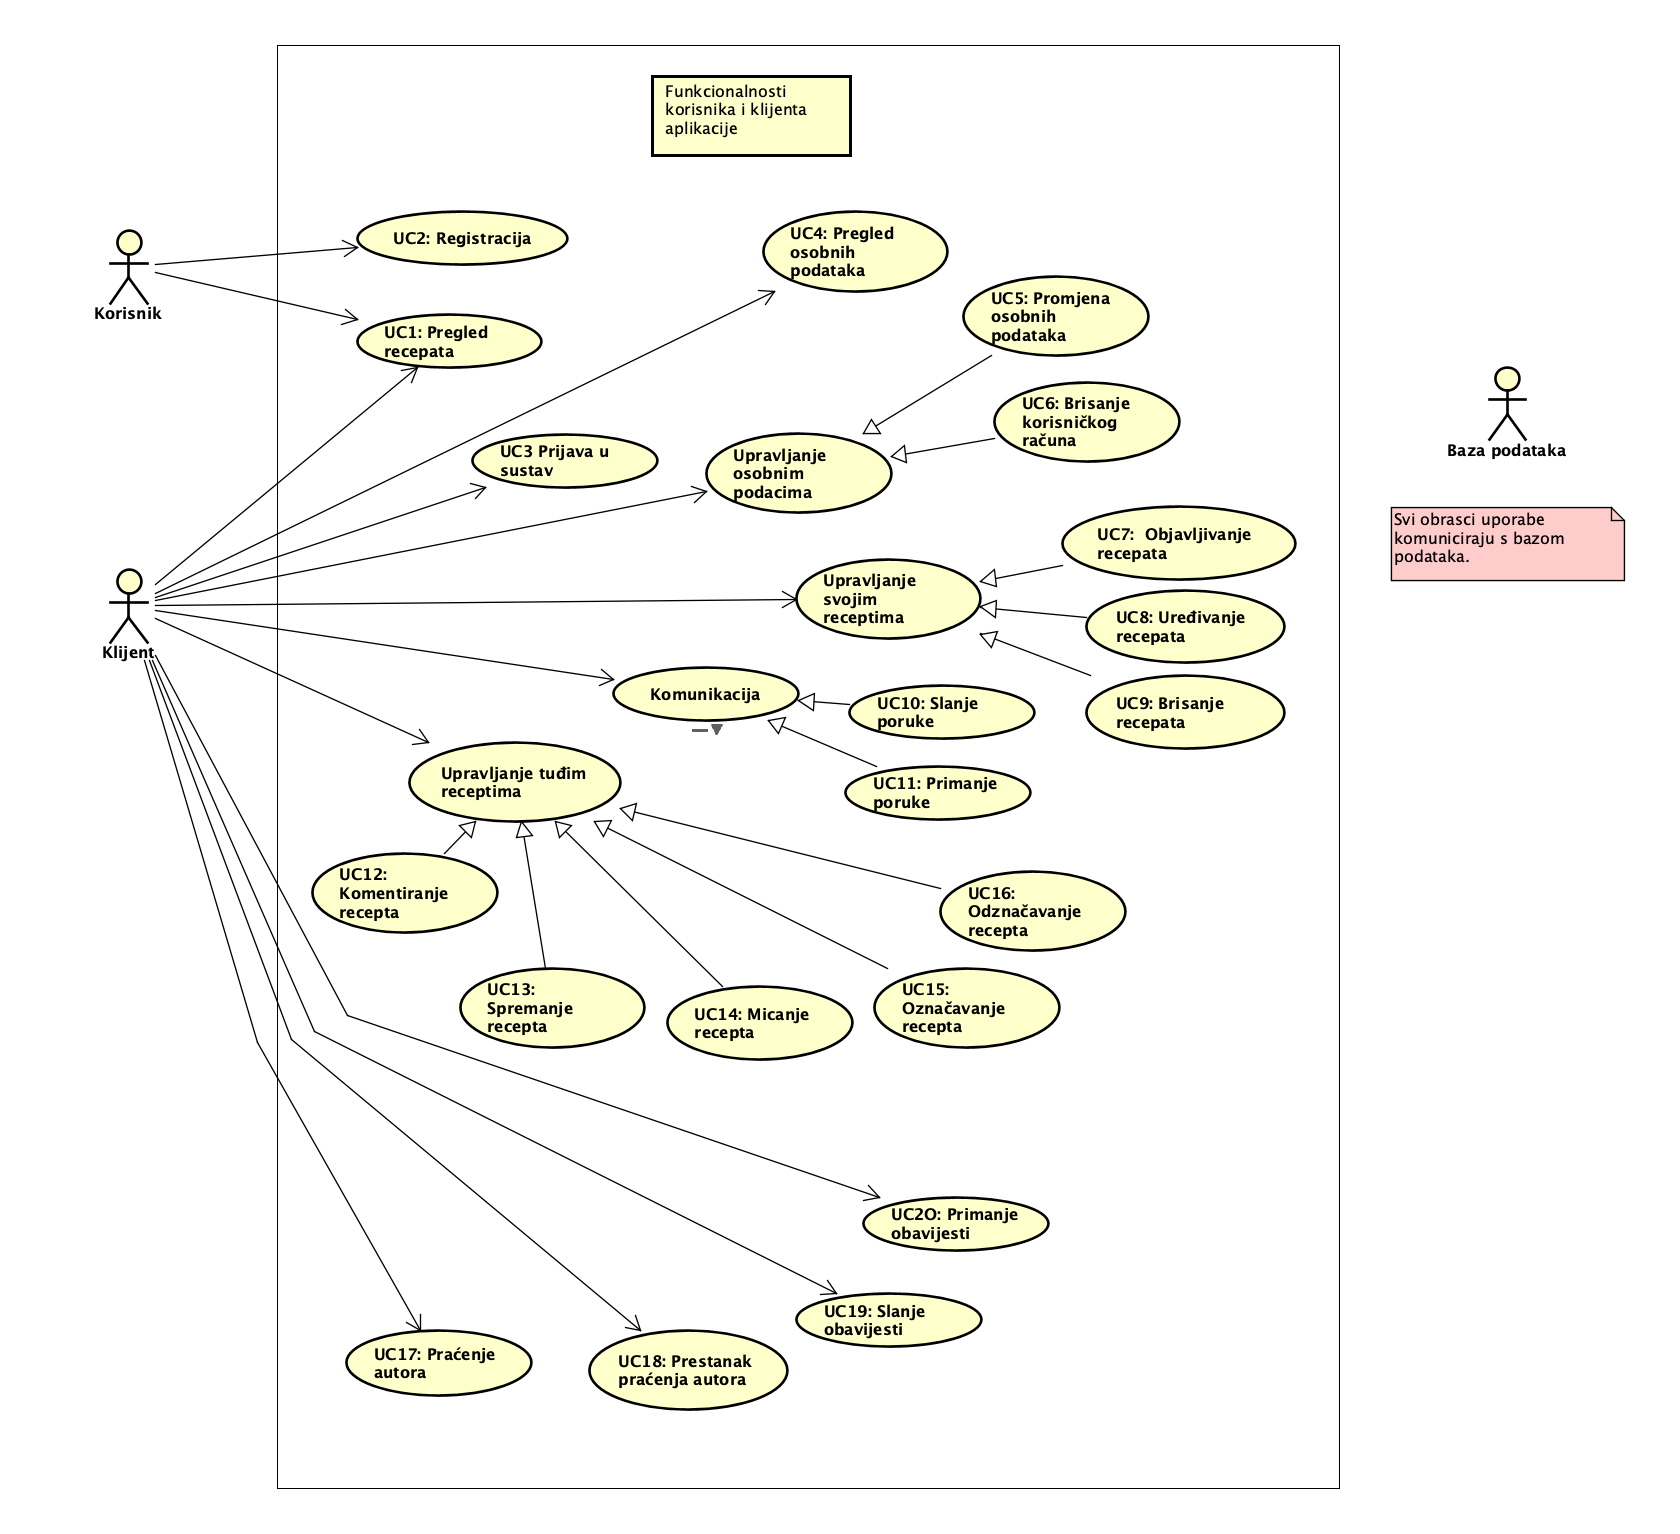
\includegraphics[scale=0.1]{dijagrami/Korisnik_klijent.png} 
			\centering
			\caption{}
			\label{fig:id1}
		\end{figure}
		\begin{figure}[H]
			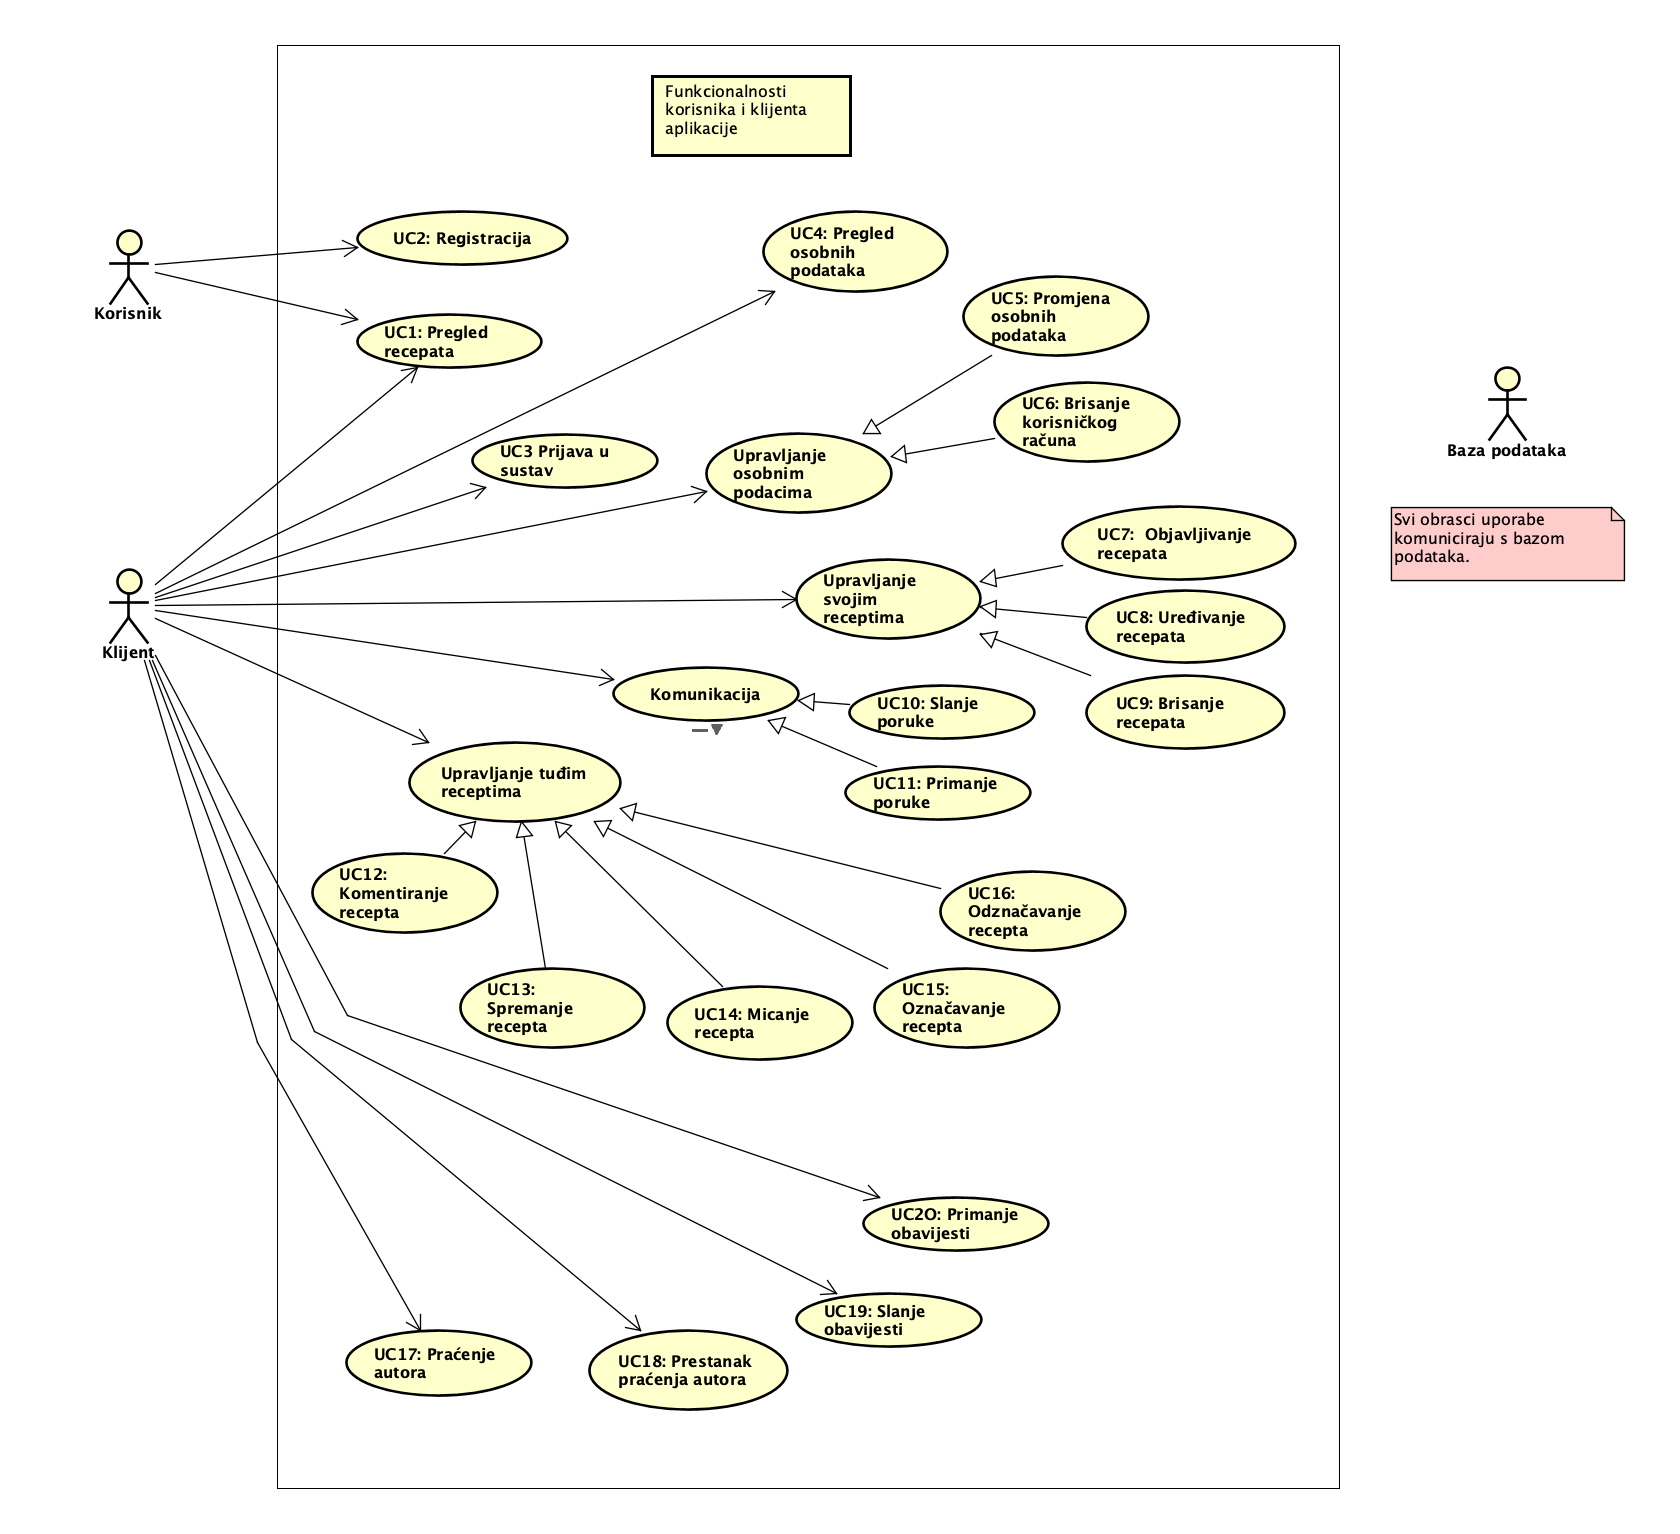
\includegraphics[scale=0.1]{dijagrami/Korisnik_klijent.png} 
			\centering
			\caption{}
			\label{fig:id2}
		\end{figure}
		\begin{figure}[H]
			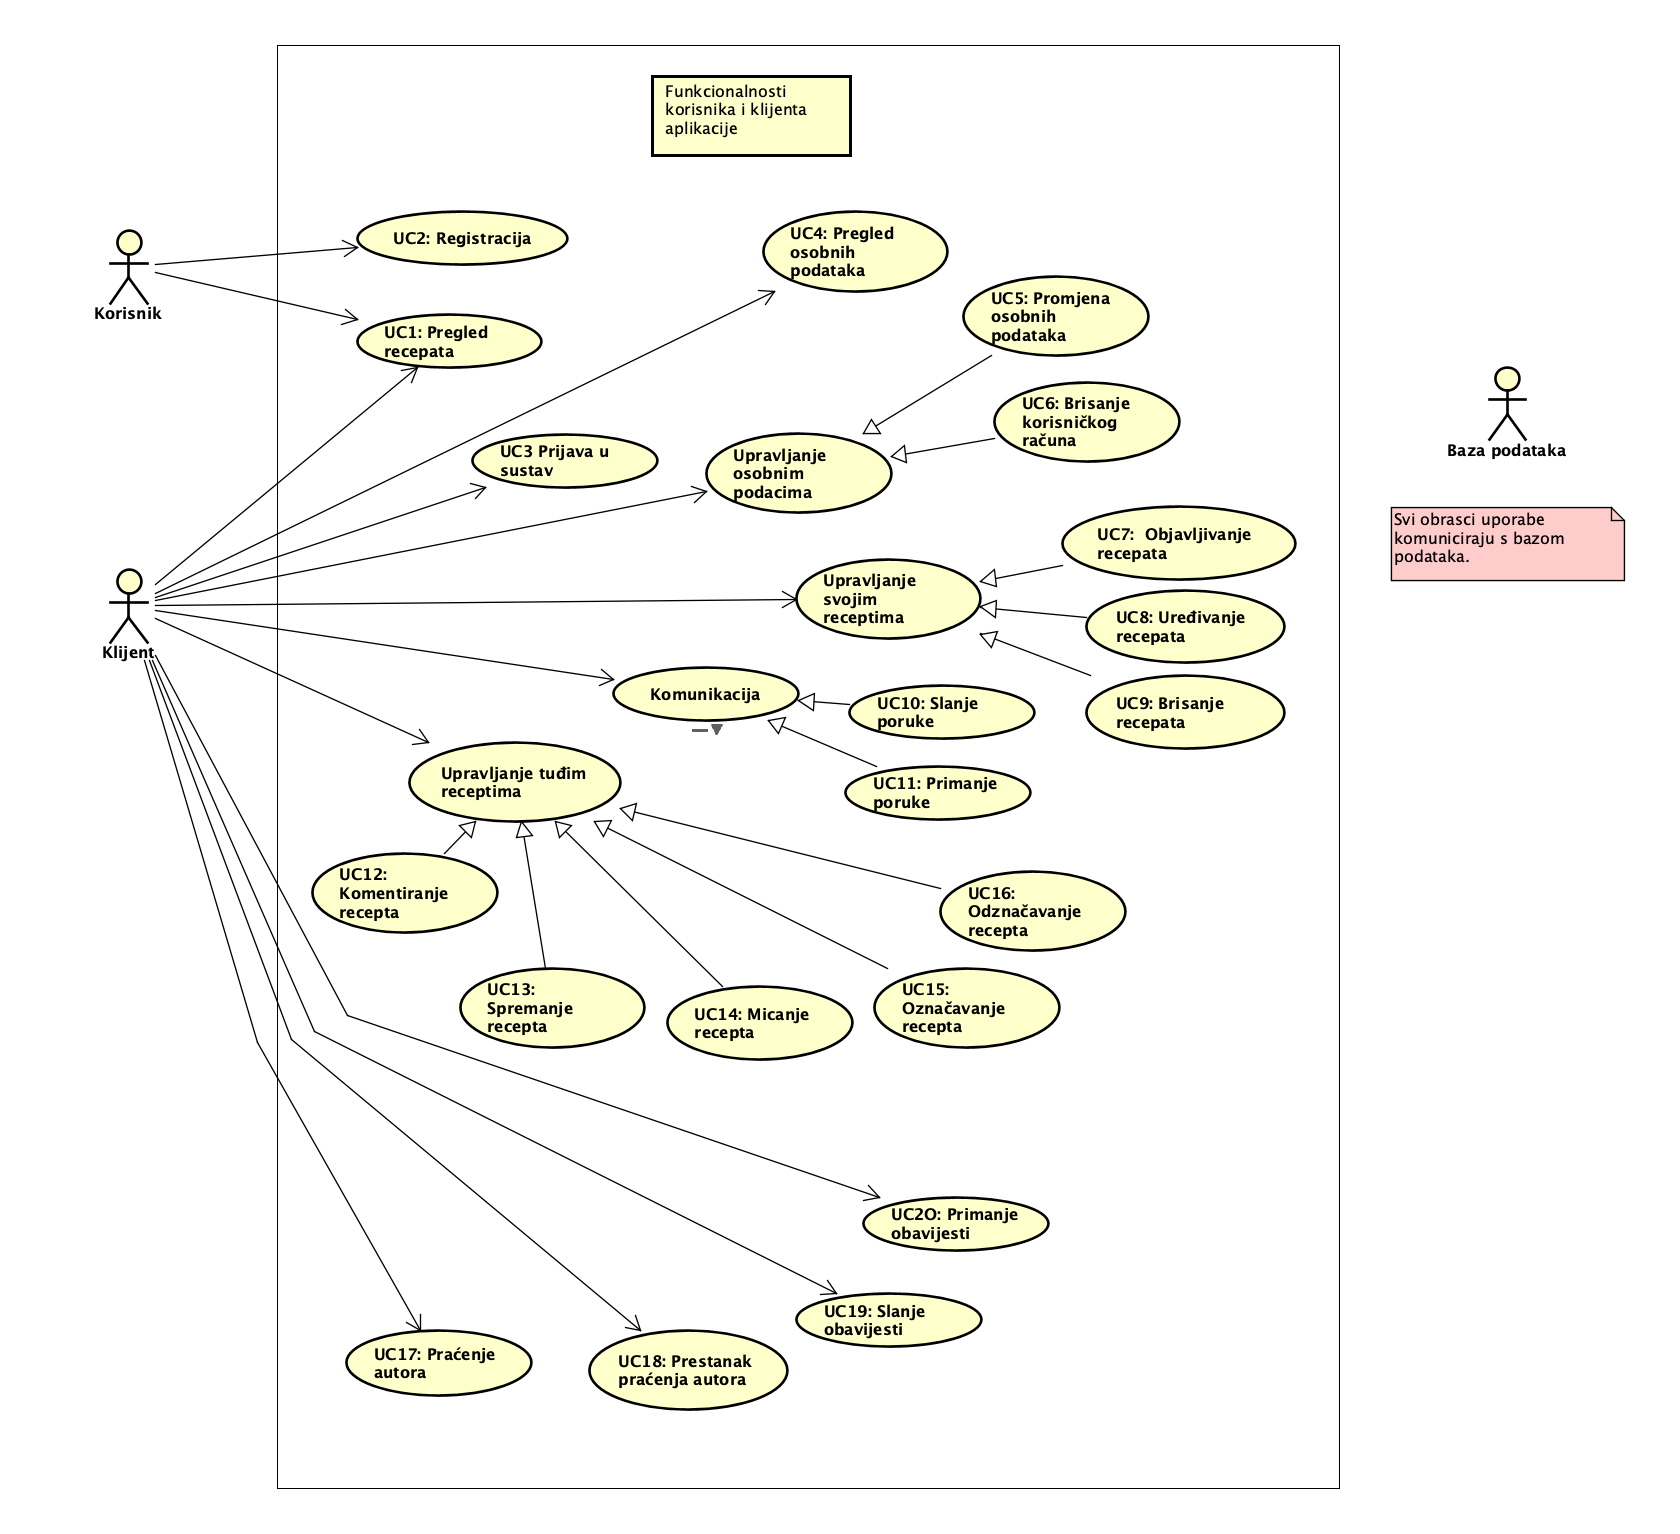
\includegraphics[scale=0.1]{dijagrami/Korisnik_klijent.png} 
			\centering
			\caption{}
			\label{fig:id3}
		\end{figure}
		\begin{figure}[H]
			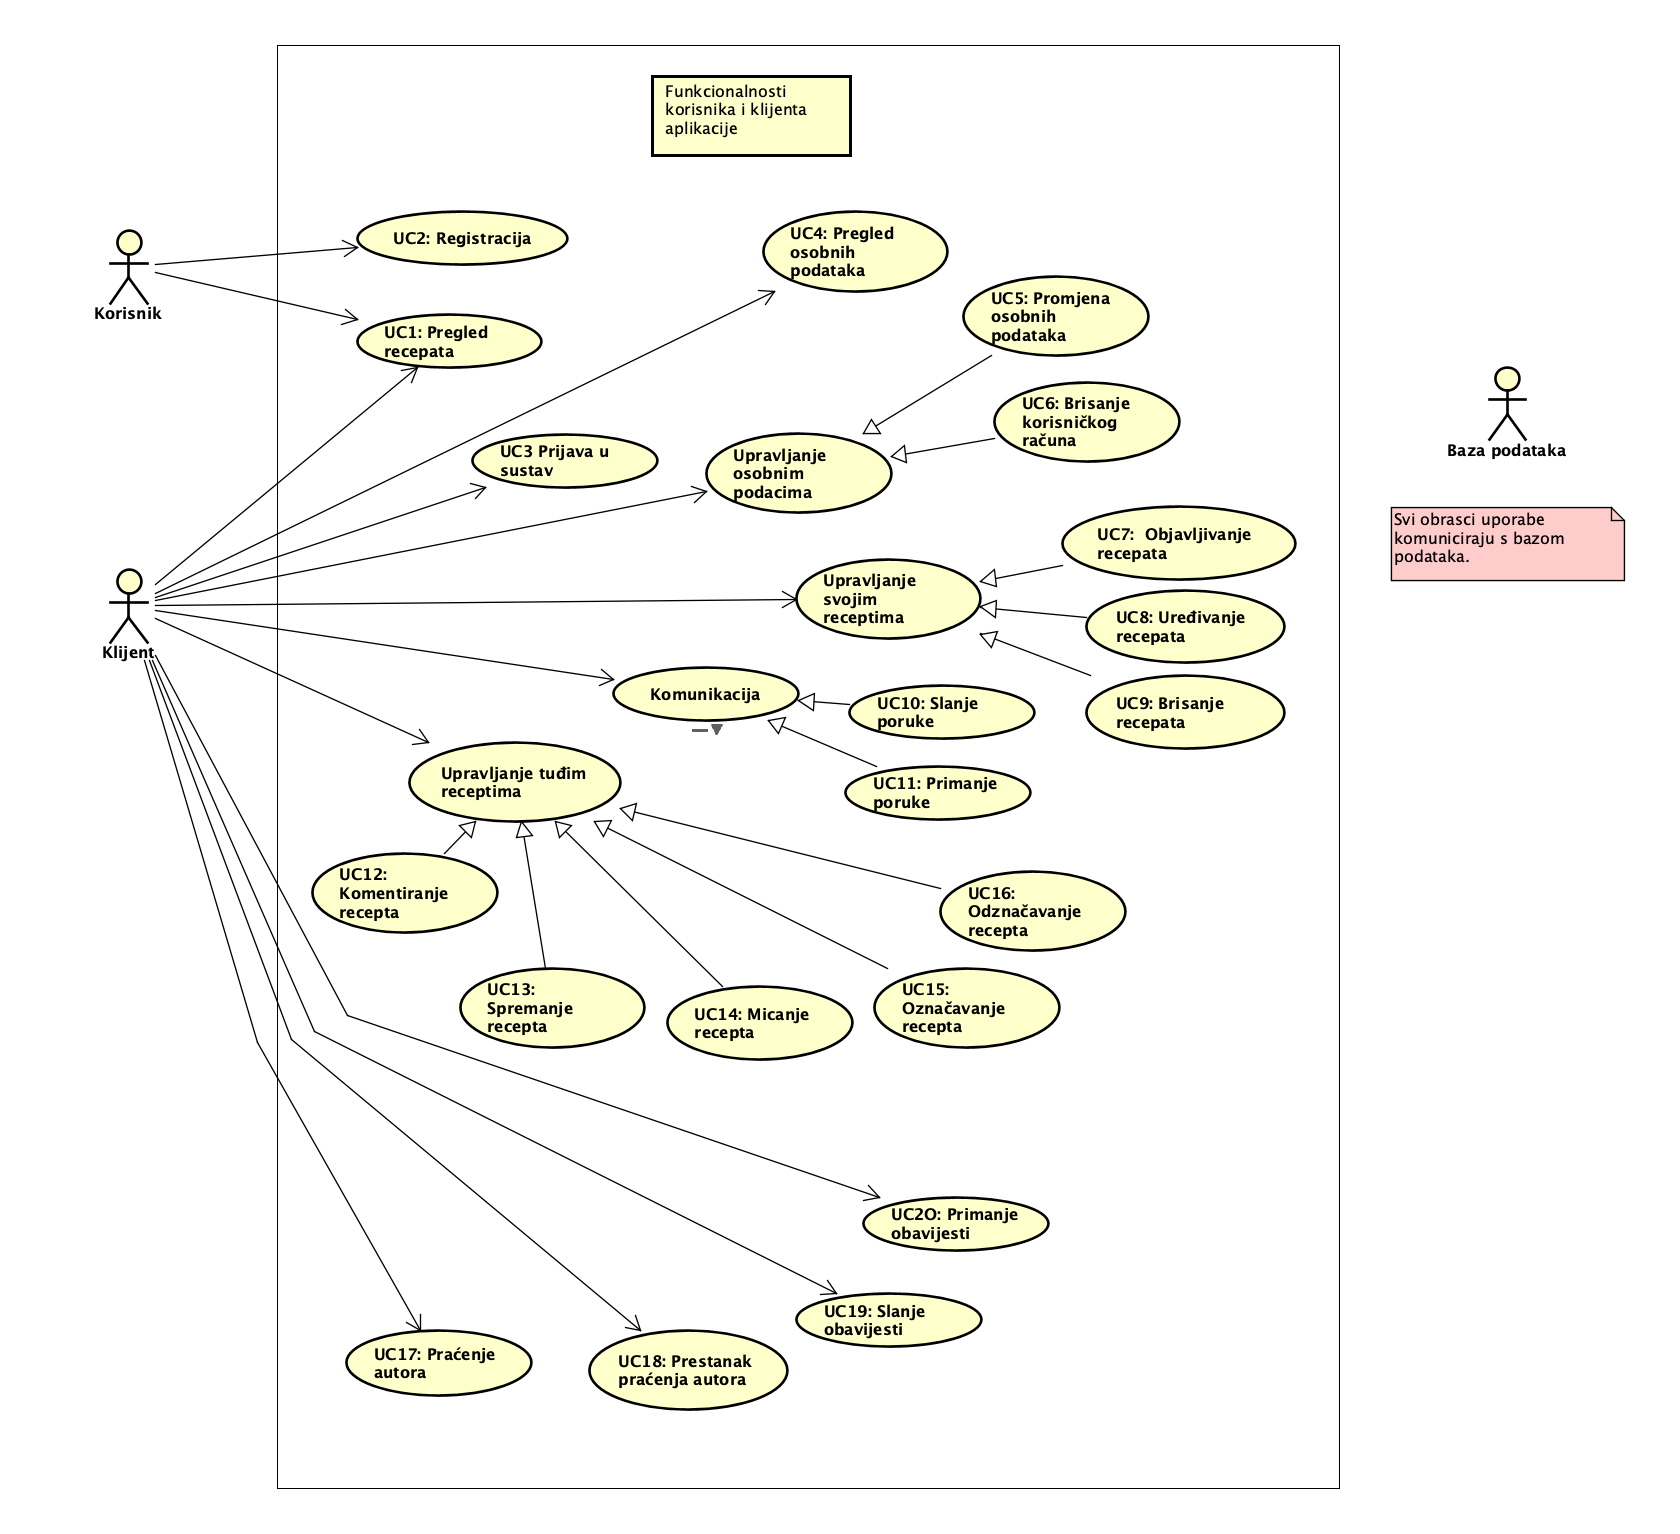
\includegraphics[scale=0.1]{dijagrami/Korisnik_klijent.png} 
			\centering
			\caption{}
			\label{fig:id4}
		\end{figure}
		\begin{figure}[H]
			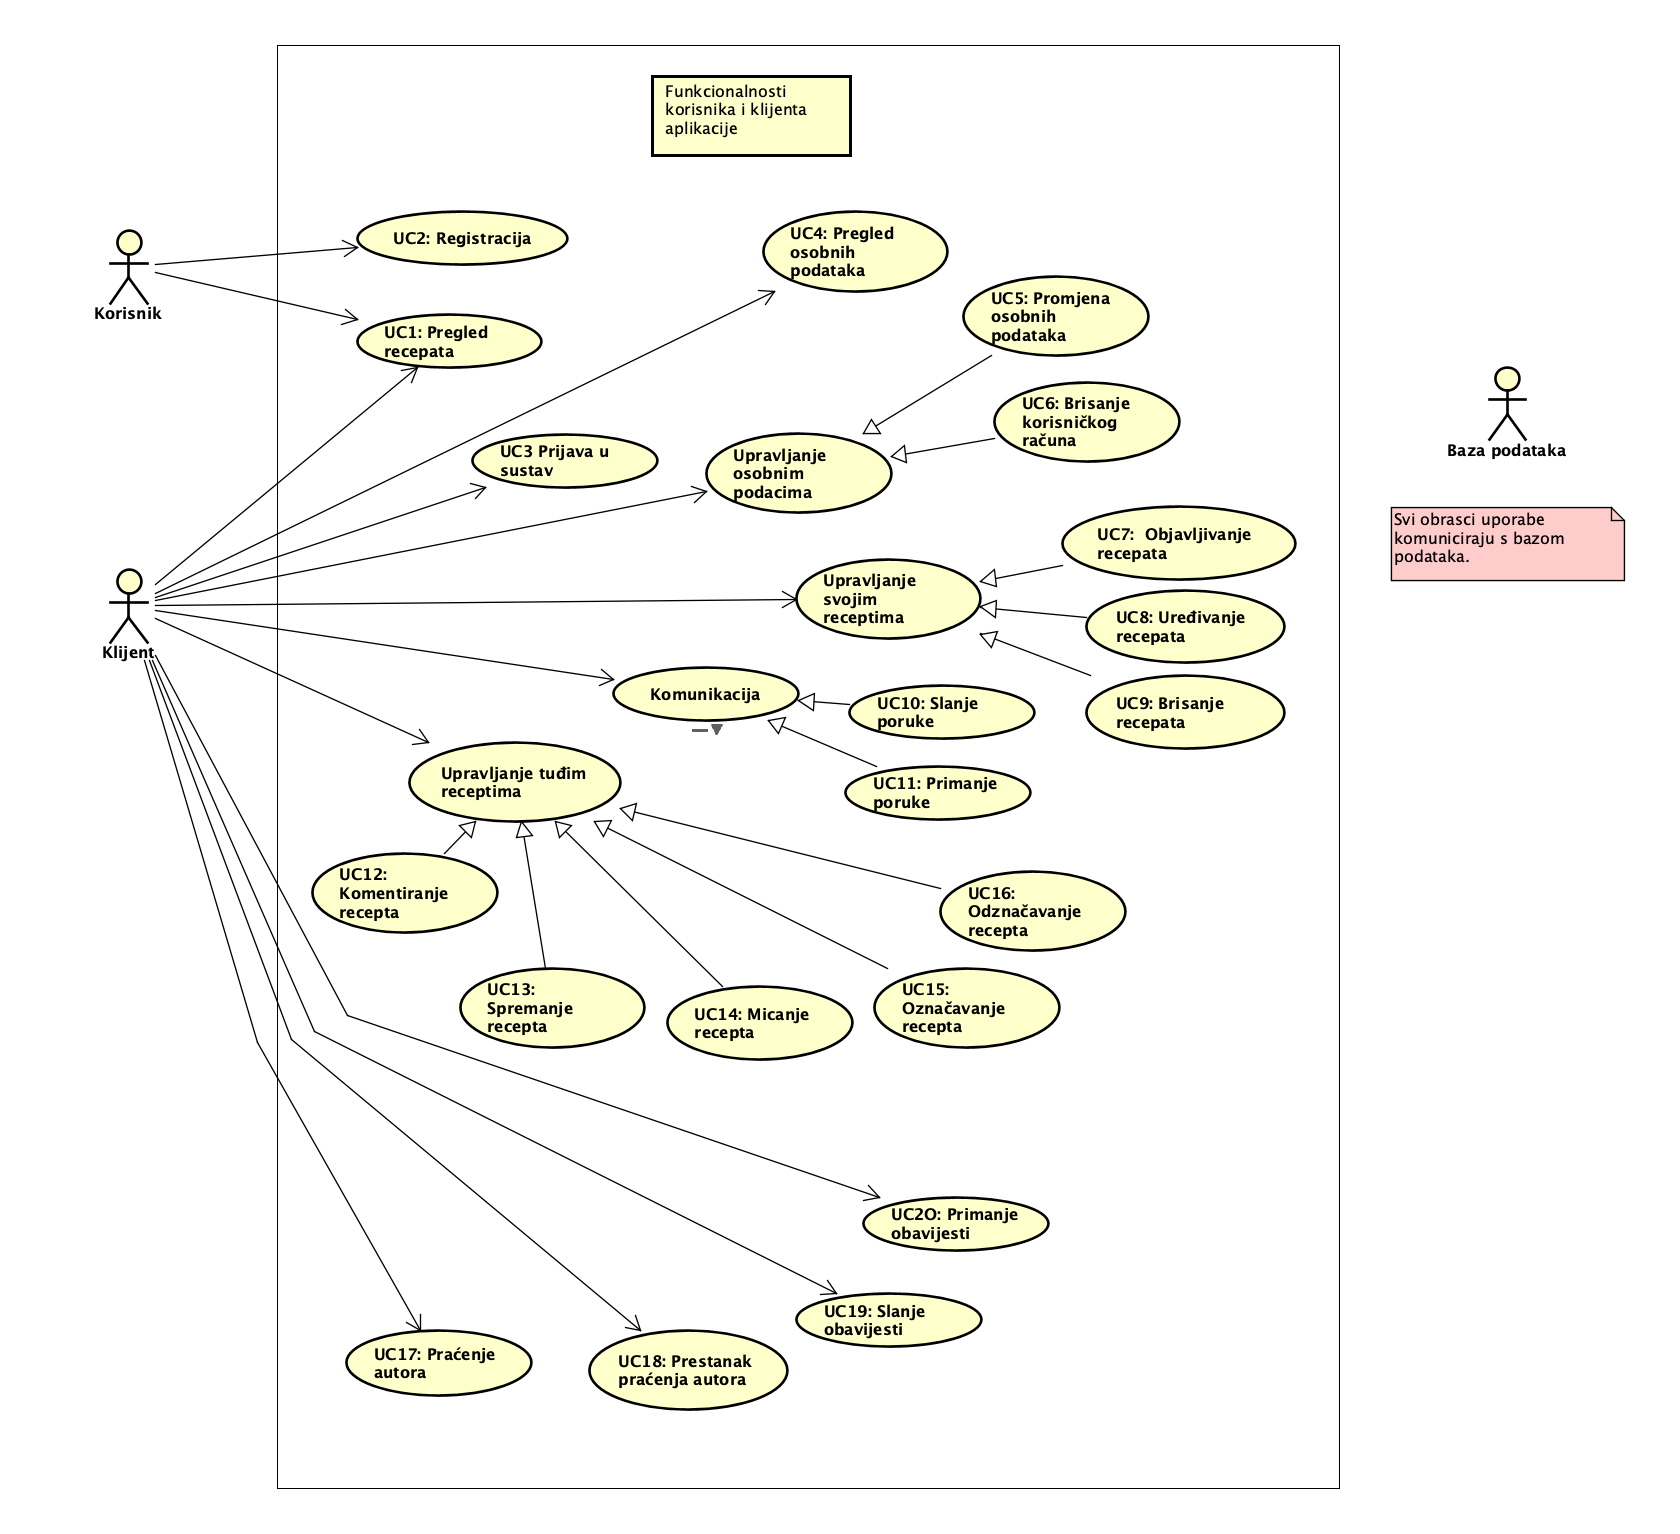
\includegraphics[scale=0.1]{dijagrami/Korisnik_klijent.png} 
			\centering
			\caption{}
			\label{fig:id5}
		\end{figure}
		\begin{figure}[H]
			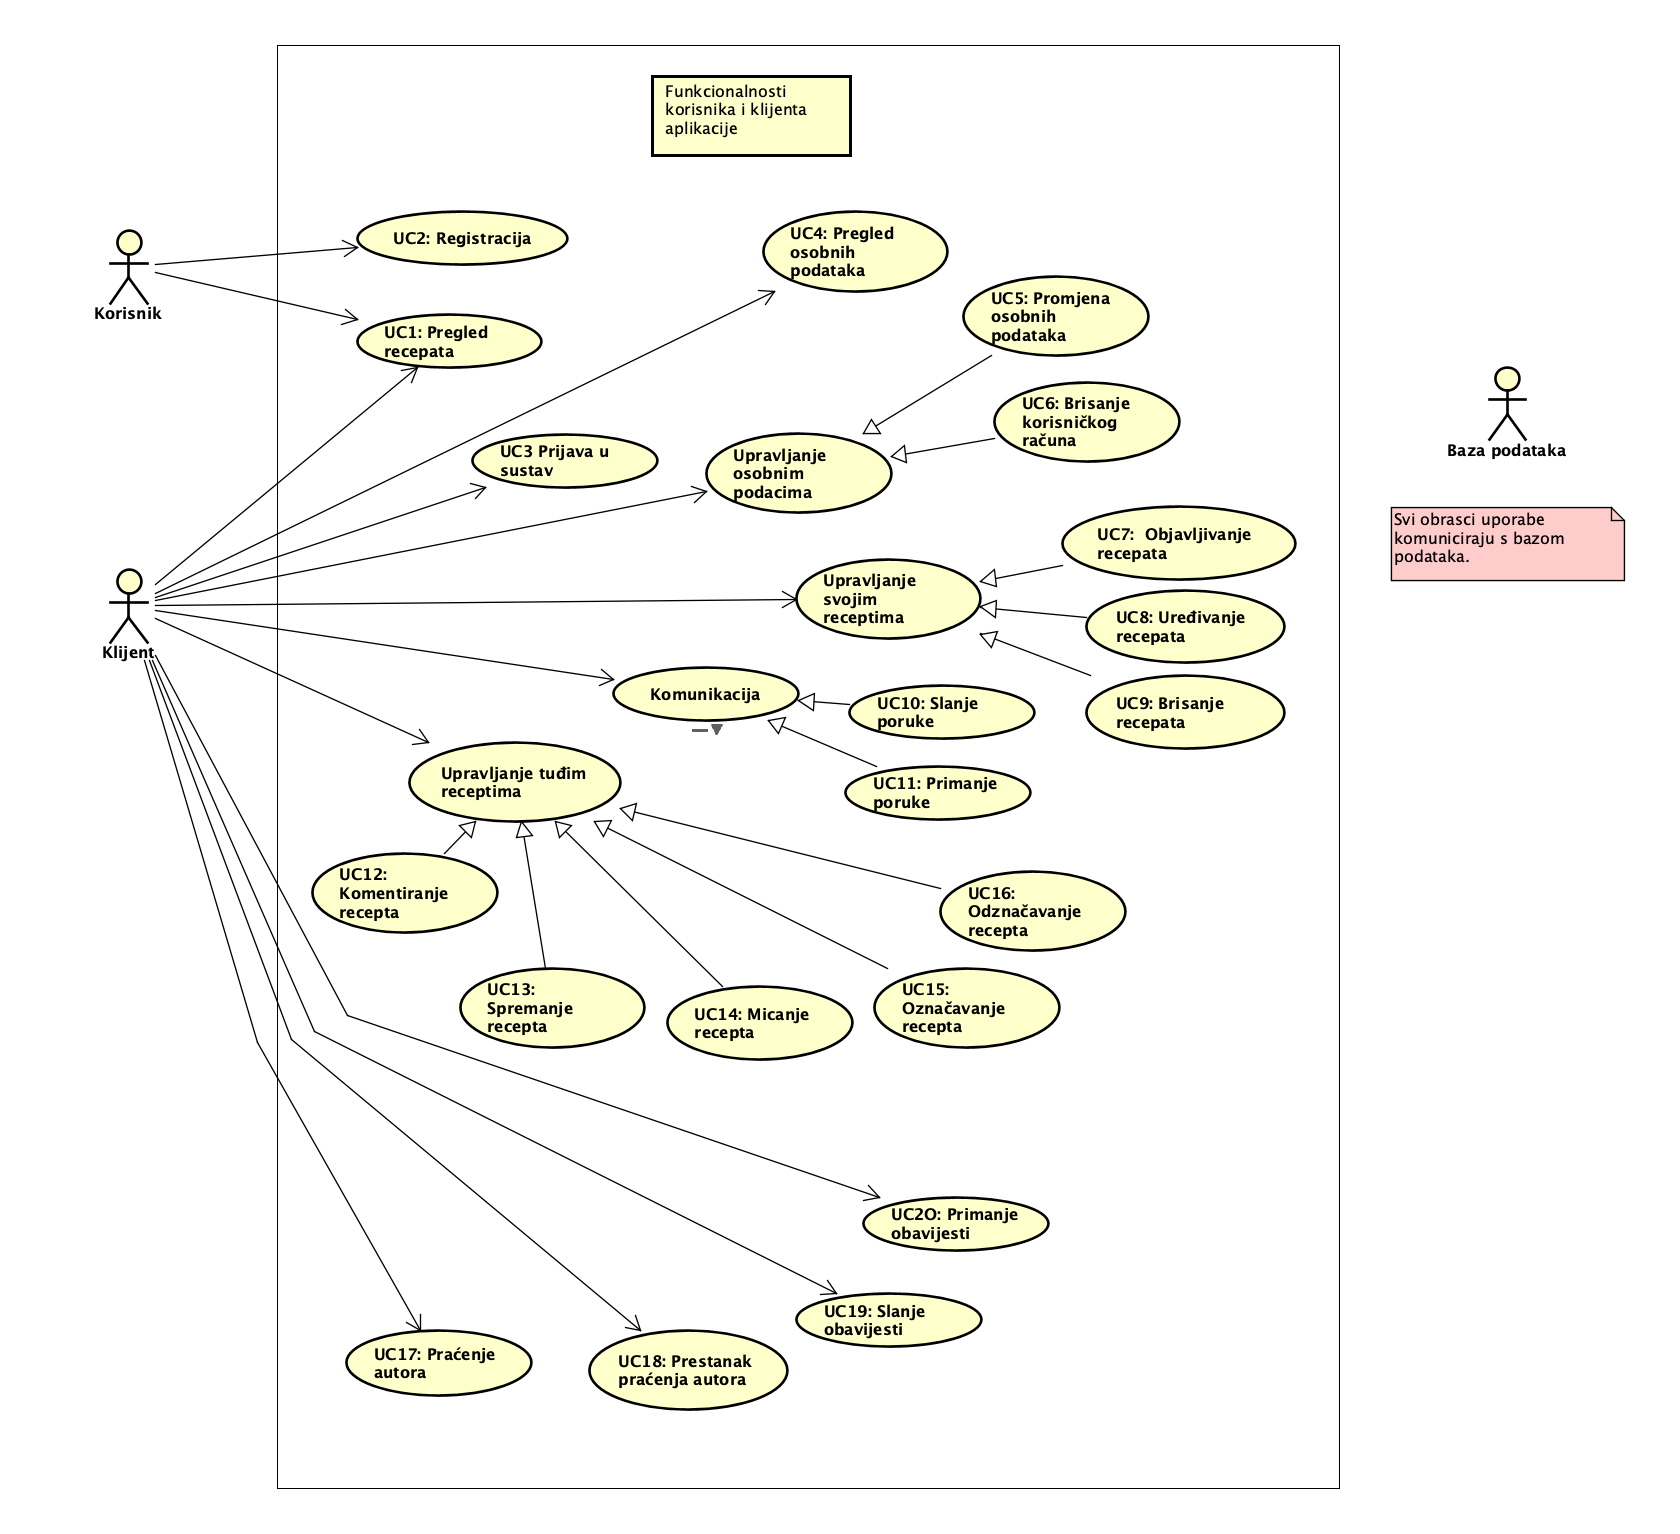
\includegraphics[scale=0.1]{dijagrami/Korisnik_klijent.png} 
			\centering
			\caption{}
			\label{fig:id6}
		\end{figure}